\chapter{2 models for \((\infty,1)\)-categories}

In this part, we introduce two models for \((\infty,1)\)-categories. One is based on simplicial sets satisfying certain horn extension properties, the other is based on simplicial categories. These two models come with two model structure respectively, and the coherent nerve construction of Cordier can be used to show that they are Quillen equivalent.

\section{Basics on \(\infty\)-categories}

Let us first introduce some basic notions related to simplicial sets.
\begin{definition}[Category of finite ordinals]
    We define a category \(\Delta\) as follows:
    \begin{enumerate}
        \item The objects are linearly order sets of the form \([n]\) for every integer \(n\geq 0\)
              \[[n]:=(0<1<\cdots<n).\]
        \item Given \(m,n\geq 0\), a morphism \(f:[m]\rightarrow [n]\) in \(\Delta\) is an order-preserving map. Said differently, for any \(0\leq i\leq j\leq m\), we have \(0\leq f(i)\leq f(j)\leq n\).
    \end{enumerate}
\end{definition}

There are two important classes of maps: one is the unique coface map
\[d^k:[n-1]\rightarrow [n],\ \ \ 0\leq k\leq n\]
which does not have \(k\) in its image and is injective. The other is the unique codegeneracy map
\[s^k:[n+1]\rightarrow [n],\ \ \ 0\leq k\leq n\]
which hits \(k\) twice and is surjective. They satisfy a list of cosimplicial identities, see~\cite{goerssSimplicialHomotopyTheory2009}. Now we define the simplicial sets as contravariant functors.

\begin{definition}[Simplicial sets]
    A \textbf{simplicial set} \(X\) is a contravariant functor \(X:\Delta^{op}\rightarrow \mathcal{Sets}\). They form a category where the morphisms are natural transformations. For a simplicial set \(X\), we write \(X_n:=X([n])\) as its values. The face maps are \(d_k=X(d^k)\) and the degeneracy maps are \(s_k=X(s^k)\). They satisfy the corresponding simplicial identities.
\end{definition}

We can associate a simplicial set to a category using the nerve construction. For each fixed \(n\geq 0\), we can view \([n]\) as a category as follows:
\begin{itemize}
    \item We have \(n+1\) objects: the number \(0,1,\ldots,n\).
    \item For \(0\leq i\leq j\leq n\), we have a unique morphism \(i\rightarrow j\) (if \(i=j\), this is the unique identity morphism of \(i\)). The composition of morphisms is given by the transitivity of \(\leq\).
\end{itemize}

\begin{example}
    Let \(\mathcal{C}\) be a category. The nerve of \(\mathcal{C}\) is a simplicial set \(N(\mathcal{C})\) given by
    \[N(\mathcal{C})_n:=\text{Fun}([n],\mathcal{C})\]
    for each \(n\geq 0\). Namely, all functors from the category \([n]\) to the category \(\mathcal{C}\). Here \(N(\mathcal{C})_n\) can be viewed as a string of \(n\) composable morphisms in \(\mathcal{C}\):
    \[C_0\xrightarrow{f_1}C_1\xrightarrow{f_2}\cdots\xrightarrow{f_{n}}C_n\]
    As a special case, consider \(\mathcal{C}=\Delta\). Fix \(n\geq 0\), the nerve \(N([n])\) is a simplicial set. For every \(m\geq 0\), we have
    \[N([n])_m=\text{Fun}([m],[n])=\hom_\Delta([m],[n]).\]
    Because the functors from the category \([m]\) to \([n]\) are exactly the morphism from \([m]\) to \([n]\) if we view them as objects in \(\Delta\). This simplicial set \(N([n])=\hom_\Delta(-,[n])\) is usually denoted as \(\Delta^n\), which is the simplicial set represented by \([n]\in \Delta\).

    Given a simplicial set \(X\), by the Yoneda lemma, the simplicial maps \(\Delta^n\rightarrow X\) classify \(n\)-simplices of \(X\) in the sense that we have a natural bijection
    \[\hom_{\mathcal{sSet}}(\Delta^n,X)\cong X_n.\]
\end{example}

Let \(\mathcal{C}\) be a category. The vertices \(N(\mathcal{C})_0\) in the simplicial set \(N(\mathcal{C})\) can be viewed as objects in \(\mathcal{C}\) and the edges \(N(\mathcal{C})_1\) can be viewed as morphisms in \(\mathcal{C}\). Consider the following triangle in the \([2]\):
% https://q.uiver.app/#q=WzAsMyxbMSwwLCIxIl0sWzAsMSwiMCJdLFsyLDEsIjIiXSxbMSwwXSxbMCwyXSxbMSwyXV0=
\[\begin{tikzcd}
        & 1 \\
        0 && 2
        \arrow[from=1-2, to=2-3]
        \arrow[from=2-1, to=1-2]
        \arrow[from=2-1, to=2-3]
    \end{tikzcd}\]
\(N(\mathcal{C})_2\) consists of functors defined on the above triangle. The face map \(d_1:N(\mathcal{C})_2\rightarrow N(C)_1\) is essentially given by composition: how we can compose two morphism into one morphism in \(\mathcal{C}\). Strictly speaking, a 2-simplex in \(N(\mathcal{C})\) is a pair of composable morphisms together with their composition.

Now let \(\mathcal{Cat}\) be the category of categories and \(\mathcal{sSet}\) be the category of simplicial sets.

\begin{lemma}
    The nerve functor \(N:\mathcal{Cat}\rightarrow \mathcal{sSet}\) is fully faithful and hence induces an equivalence onto its essential image.
\end{lemma}
\begin{proof}
    The full proof can be found at~\cite[\href{https://kerodon.net/tag/002Z}{Tag 002Z}]{lurieKerodon2025}. We only give a sketch here.
\end{proof}

Our next goal is to understand the essential image. We next introduce two construction from \(\Delta^n\). \(\Delta^n\) contains two subcomplexes: the boundary \(\partial \Delta^n\) and the \(k\)-th horn \(\Lambda^n_k\). It is not hard to see that the boundary \(\partial \Delta^n\) can be identified with the coequalizer
\[\bigsqcup_{0\leq i<j\leq n} \Delta^{n-2}\rightrightarrows \bigsqcup_{i=0}^n \Delta^{n-1}\rightarrow \partial \Delta^n.\]
The \(k\)th \(n\)-horn \(\Lambda_k^n\subseteq \partial \Delta^n\) for \(0\leq k\leq n\) is obtained from \(\partial \Delta^n\) by removing the \(k\)th face: the face opposite to the vertex \(k\). The \(k\)th horn can also be identified with the coequalizer:
\[\bigsqcup_{0\leq i<j\leq n} \Delta^{n-2}\rightrightarrows \bigsqcup_{i\neq k} \Delta^{n-1}\rightarrow \Lambda^n_k.\]

\begin{example}
    Assume the dimension \(n=2\) and \(\mathcal{C}\) is a category. We have 3 different horns \(\Lambda^2_k\rightarrow N(\mathcal{C})\) for \(0\leq k\leq 2\). From our previous discussion on nerves, we know that they look like the following:
    % https://q.uiver.app/#q=WzAsOSxbMCwxLCJjXzAiXSxbMiwxLCJjXzIiXSxbMSwwLCJjXzEiXSxbMywxLCJjXzAiXSxbNSwxLCJjXzIiXSxbNCwwLCJjXzEiXSxbNiwxLCJjXzAiXSxbOCwxLCJjXzIiXSxbNywwLCJjXzEiXSxbMCwyLCJmIl0sWzAsMSwiaCIsMl0sWzMsNSwiZiJdLFs1LDQsImciXSxbNiw3LCJoIiwyXSxbOCw3LCJnIl1d
    \[\begin{tikzcd}
            & {c_1} &&& {c_1} &&& {c_1} \\
            {c_0} && {c_2} & {c_0} && {c_2} & {c_0} && {c_2}
            \arrow["g", from=1-5, to=2-6]
            \arrow["g", from=1-8, to=2-9]
            \arrow["f", from=2-1, to=1-2]
            \arrow["h"', from=2-1, to=2-3]
            \arrow["f", from=2-4, to=1-5]
            \arrow["h"', from=2-7, to=2-9]
        \end{tikzcd}\]
    Here \(c_0,c_1,c_2\) are objects in \(\mathcal{C}\), and \(f,g,h\) are morphisms in \(\mathcal{C}\). The composition \(h=g\circ f\) in \(\mathcal{C}\) uniquely extends the any horn \(\Lambda^2_1\rightarrow N(\mathcal{C})\) to an entire 2-simplex \(\sigma:\Delta^2\rightarrow N(\mathcal{C})\), i.e., there is a unique dashing arrow making the diagram
    % https://q.uiver.app/#q=WzAsMyxbMCwwLCJcXExhbWJkYV4yXzEiXSxbMSwwLCJOKFxcbWF0aGNhbHtDfSkiXSxbMCwxLCJcXERlbHRhXjIiXSxbMCwyXSxbMCwxXSxbMiwxLCJcXGV4aXN0cyAhIiwyLHsic3R5bGUiOnsiYm9keSI6eyJuYW1lIjoiZGFzaGVkIn19fV1d
    \[\begin{tikzcd}
            {\Lambda^2_1} & {N(\mathcal{C})} \\
            {\Delta^2}
            \arrow[from=1-1, to=1-2]
            \arrow[from=1-1, to=2-1]
            \arrow["{\exists !\sigma}"', dashed, from=2-1, to=1-2]
        \end{tikzcd}\]
    commute. The composition \(h=g\circ f\) is given by the new face \(d_1(\sigma):\Delta^1\rightarrow N(\mathcal{C})\). Next, we consider the horn \(\Lambda^2_0\rightarrow N(\mathcal{C})\), the existence of the extension \(c_1\rightarrow c_2\) is equivalent to \(f\) has a left inverse in \(\mathcal{C}\). Similar observations can be made to \(\Lambda^2_2\rightarrow N(\mathcal{C})\).
\end{example}
The above example leads us to the following definition:
\begin{definition}[Inner horns and outer horns]
    Given \(n\geq 0\), the horns \(\Lambda^n_k\subseteq \Delta^n\) for \(0<k<n\) are called \textbf{inner horns} and \(\Lambda^n_0\) and \(\Lambda^n_n\) are called \textbf{outer horns}.
\end{definition}
It turns out that the extension properties in the above example describe the essential image of the nerve functor. Let \(\mathcal{Grpd}\) be the category of groupoids, where every morphism is invertible.
\begin{proposition}
    Let \(X\) be a simplicial set.
    \begin{enumerate}[(i)]
        \item There is an isomorphism \(X\cong N(\mathcal{C})\) for some \(\mathcal{C}\in \mathcal{Cat}\) if and only if every inner horn \(\Lambda^n_k\rightarrow X\), \(0<k<n\), can be uniquely extended to an \(n\)-simplex \(\Delta^n\rightarrow X\).
        \item There is an isomorphism \(X\cong N(\mathcal{G})\) for some \(\mathcal{G}\in \mathcal{Gprd}\) if and only if every horn \(\Lambda^n_k\rightarrow X\), \(0\leq k\leq n\) can be uniquely extended to an \(n\)-simplex \(\Delta^n\rightarrow X\).
    \end{enumerate}
\end{proposition}
This is very similar to the definition of Kan complex.
\begin{definition}[Kan complex]
    A simplicial set \(X\) is a \textbf{Kan complex} if every horn \(\Lambda^n_k\rightarrow X\) for \(0\leq k\leq n\) can be extended to an \(n\)-simplex \(\Delta^n\rightarrow X\).
\end{definition}
\begin{remark}
    Note that for Kan complexes, the extension is not unique, unlike for the nerves of categories. We do not want uniqueness in the definition of \(\infty\)-categories. The composition of morphisms, in some sense, is not strictly unique, but only up to 'homotopy'.
\end{remark}
Let \(\mathcal{Kan}\subseteq \mathcal{sSet}\) be the full subcategory spanned by the Kan complexes. We have the following commutative diagram of fully faithful functors
% https://q.uiver.app/#q=WzAsNCxbMCwwLCJcXG1hdGhjYWx7R3JwZH0iXSxbMSwwLCJcXG1hdGhjYWx7Q2F0fSJdLFswLDEsIlxcbWF0aGNhbHtLYW59Il0sWzEsMSwiXFxtYXRoY2Fse3NTZXR9Il0sWzAsMiwiTiIsMl0sWzEsMywiTiJdLFswLDFdLFsyLDNdXQ==
\[\begin{tikzcd}
        {\mathcal{Grpd}} & {\mathcal{Cat}} \\
        {\mathcal{Kan}} & {\mathcal{sSet}}
        \arrow[from=1-1, to=1-2]
        \arrow["N"', from=1-1, to=2-1]
        \arrow["N", from=1-2, to=2-2]
        \arrow[from=2-1, to=2-2]
    \end{tikzcd}\]
Now we can define the \(\infty\)-categories.
\begin{definition}[\(\infty\)-categories]
    A simplicial set \(\mathcal{C}\) is an \textbf{\(\infty\)-category} if every inner horn \(\Lambda^n_k\rightarrow \mathcal{C}\) for \(0<k<n\) can be extended be an \(n\)-simplex \(\Delta^n\rightarrow \mathcal{C}\).
\end{definition}
Any ordinary category \(\mathcal{C}\) gives rise to an \(\infty\)-category \(N(\mathcal{C})\). There exists interesting \(\infty\)-categories not of this form. In particular, every simplicial model category has an underlying \(\infty\)-category. Let us first introduce some basic terminology for \(\infty\)-categories. They are similar to the nerves we discussed before.

Let \(\mathcal{C}\) be an \(\infty\)-category.
\begin{itemize}
    \item The objects are the vertices \(x\in \mathcal{C}_0\), and the morphisms are \(1\)-simplices \(f\in \mathcal{C}_1\).
    \item We have the face maps
          \begin{align*}
              s=d_1: & \mathcal{C}_1\rightarrow \mathcal{C}_0, \\
              t=d_0: & \mathcal{C}_1\rightarrow \mathcal{C}_0
          \end{align*}
          where \(s\) sends a morphism to its source, and \(t\) to its target. More formally, we define the set of morphisms for objects \(x,y\) as the pullback square
          % https://q.uiver.app/#q=WzAsNCxbMCwwLCJcXGhvbV9cXG1hdGhjYWx7Q30oeCx5KSJdLFswLDEsIioiXSxbMSwxLCJcXG1hdGhjYWx7Q31fMFxcdGltZXNcXG1hdGhjYWx7Q31fMCJdLFsxLDAsIlxcbWF0aGNhbHtDfV8xIl0sWzAsMV0sWzAsM10sWzMsMiwiKHMsdCkiXSxbMSwyLCIoeCx5KSIsMl1d
          \[\begin{tikzcd}
                  {\hom_\mathcal{C}(x,y)} & {\mathcal{C}_1} \\
                  {*} & {\mathcal{C}_0\times\mathcal{C}_0}
                  \arrow[from=1-1, to=1-2]
                  \arrow[from=1-1, to=2-1]
                  \arrow["{(s,t)}", from=1-2, to=2-2]
                  \arrow["{(x,y)}"', from=2-1, to=2-2]
              \end{tikzcd}\]
    \item The degeneracy map 
          \[id=s_0:\mathcal{C}_0\rightarrow \mathcal{C}_1\]
          is the identity map.
\end{itemize}
Let us take a closer look at the composition for \(\mathcal{C}\). Consider two morphisms \(f:x\rightarrow y\) and \(g:y\rightarrow z\). These morphisms together define an inner horn:
\[\lambda=(g,\cdot,f):\Lambda^2_1\rightarrow \mathcal{C}\]
% https://q.uiver.app/#q=WzAsMyxbMCwxLCJ4Il0sWzEsMCwieSJdLFsyLDEsInoiXSxbMCwxLCJmIl0sWzEsMiwiZyJdXQ==
\[\begin{tikzcd}
        & y \\
        x && z
        \arrow["g", from=1-2, to=2-3]
        \arrow["f", from=2-1, to=1-2]
    \end{tikzcd}\]
Here \(d_0\lambda=g\) and \(d_1\lambda=f\). By definition of the \(\infty\)-category \(\mathcal{C}\), such horn can be \textit{non-uniquely} extended to a \(2\)-simplex \(\sigma:\Delta^2\rightarrow \mathcal{C}\). The new face obtained \(d_1(\sigma)\) is then a candidate composition of \(g\) and \(f\). Note that this is not uniquely determined, unlike in ordinary categories. We only demand that any choice of such a composition is equally good: the space of all such choices is to be contractible. Later we will give a more precise statement. 

We now want to describe the homotopy category \(\t{Ho}(\mathcal{C})\) of an \(\infty\)-category \(\mathcal{C}\). From what we discuss in~\ref{AppenA}, the nerve functor has a left adjoint \(\tau_1:\mathcal{sSet}\rightarrow \mathcal{Cat}\), called the \textbf{fundamental category functor} or the \textbf{categorical realization functor}. It is given by a formula 
\[\tau_1(X)=\t{colim}_{(\delta/X)}[-]\circ p.\]
If the simplicial set \(X\) happens to be an \(\infty\)-category, there is a simple description of the fundamental category \(\tau_1(X)\). The morphisms in \(\tau_1(X)\) can be represented by actual \(1\)-simplices. We need the definition of homotopies in \(\infty\)-categories.
\begin{definition}[homotopy]
     Two morphisms \(f,g:x\rightarrow y\) in an \(\infty\)-category \(\mathcal{C}\) are homotopic (write \(f\simeq g\)) if there is a \(2\)-simplex \(\sigma:\Delta^2\rightarrow \mathcal{C}\) with boundary \(\partial \sigma=(g,f,id_x)\), i.e. the boundary looks like 
     % https://q.uiver.app/#q=WzAsMyxbMSwwLCJ4Il0sWzAsMSwieCJdLFsyLDEsInkiXSxbMSwyLCJmIl0sWzAsMiwiZyJdLFsxLDAsImlkX3giXV0=
     \[\begin{tikzcd}
             & x \\
             x && y
             \arrow["g", from=1-2, to=2-3]
             \arrow["{id_x}", from=2-1, to=1-2]
             \arrow["f", from=2-1, to=2-3]
         \end{tikzcd}\]
    Any such \(2\)-simplex \(\sigma\) is a \textbf{homotopy} from \(f\) to \(g\), denoted by \(\sigma:f\rightarrow g\). 
\end{definition}
This indeed defines an equivalence relationship for morphisms in an \(\infty\)-category.
\begin{proposition}     
     Let \(\mathcal{C}\) be an \(\infty\)-category and \(x,y\in \mathcal{C}\). The homotopy relation is an equivalence relation on \(\hom_\mathcal{C}(x,y)\). The \textbf{homotopy class} of a morphism \(f:x\rightarrow y\) is denoted by \([f]\).
\end{proposition}
\begin{proof}
    The proof relies on the horn extension property of \(\mathcal{C}\).
\end{proof}

Next, we want to define the homotopy category \(\t{Ho}(\mathcal{C})\) by passing to the homotopy classes of morphisms. We have a lot of things to check, but first, we can show that the choice of different candidate composition of the representatives, is homotopic by using the horn extension property.
\begin{figure}[h]
    \centering
    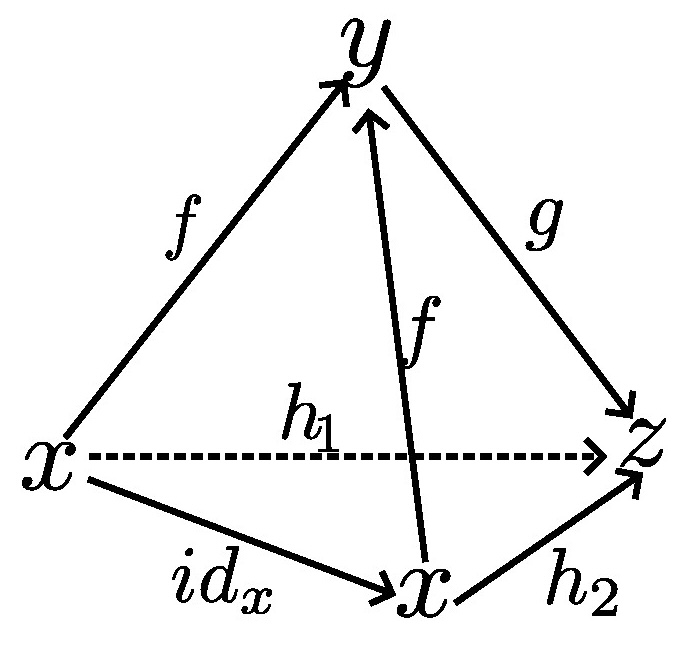
\includegraphics[width=0.3\textwidth]{tetra3.jpg}
\end{figure}


\begin{proposition}[homotopy category]
     Let \(\mathcal{C}\) be an \(\infty\)-category. There is an ordinary category \(\t{Ho}(\mathcal{C})\), the \textbf{homotopy category} of \(\mathcal{C}\), with the same objects as \(\mathcal{C}\) and morphisms the homotopy classes of morphisms in \(\mathcal{C}\). Composition and identities are given by 
     \[[g]\circ[f]=[g\circ f]\ \ \ \t{and}\ \ \ id_x:=[id_x]=[s_0x]\]
     where \(g\circ f\) is an arbitrary candidate composition of \(g\) and \(f\). Furthermore, there is a natural isomorphism of categories
     \[\t{Ho}(\mathcal{C})\cong \tau_1(\mathcal{C}).\]
\end{proposition}